\chapter{KẾT QUẢ TRIỂN KHAI VÀ XÂY DỰNG WEBSITE}

\section{Phân hệ giao diện tương tác Người dùng (Guest Web UI)}

\subsection{Trang Giới thiệu hệ thống (Landing Page)}

Trang Landing Page đóng vai trò là cửa ngõ đầu tiên chào đón người dùng truy cập vào BusGIS. Giao diện được thiết kế theo phong cách hiện đại, sử dụng hiệu ứng chuyển động mượt mà (animations) và bố cục hiển thị trực quan. Ngay từ trang chủ, hệ thống cung cấp bản đồ demo nhỏ để minh họa cho khả năng theo dõi lộ trình tuyến xe.

\begin{figure}[H]
    \centering
    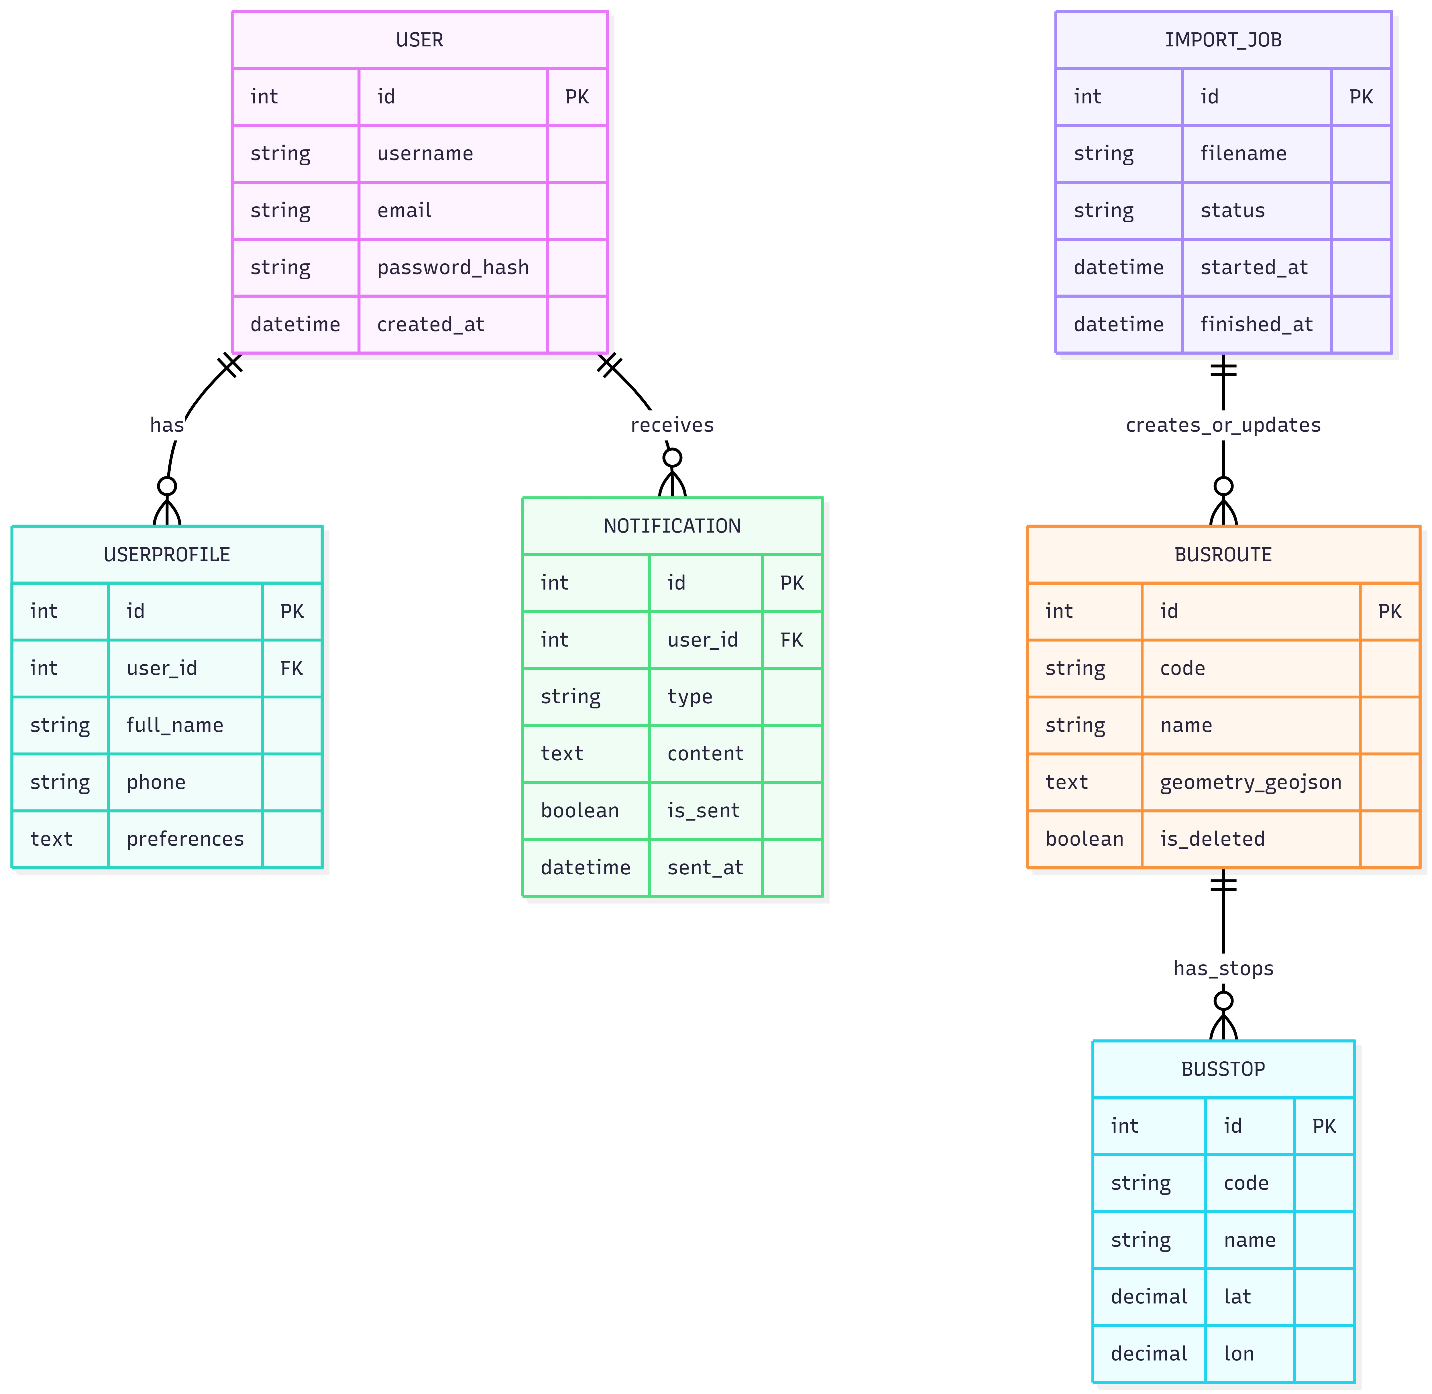
\includegraphics[width=\textwidth]{images/image4.png}
    \caption{Giao diện Trang giới thiệu hệ thống (Landing Page)}
\end{figure}

Trang cung cấp thông tin tóm tắt về số lượng tuyến, trạm hiện có và mô tả các tính năng nổi bật. Tùy thuộc vào trạng thái xác thực, hệ thống sẽ điều hướng người dùng đăng nhập hoặc truy cập trực tiếp vào hệ thống bản đồ lõi.

\subsection{Giao diện Trang chủ và nền tảng Bản đồ số}

Trung tâm của ứng dụng là Trang chủ chứa Bản đồ số tích hợp. Giao diện bản đồ được xây dựng dựa trên LeafletJS chiếm toàn bộ không gian khung hình, mang lại cảm giác trải nghiệm không giới hạn (Infinite Map View). 

\begin{figure}[H]
    \centering
    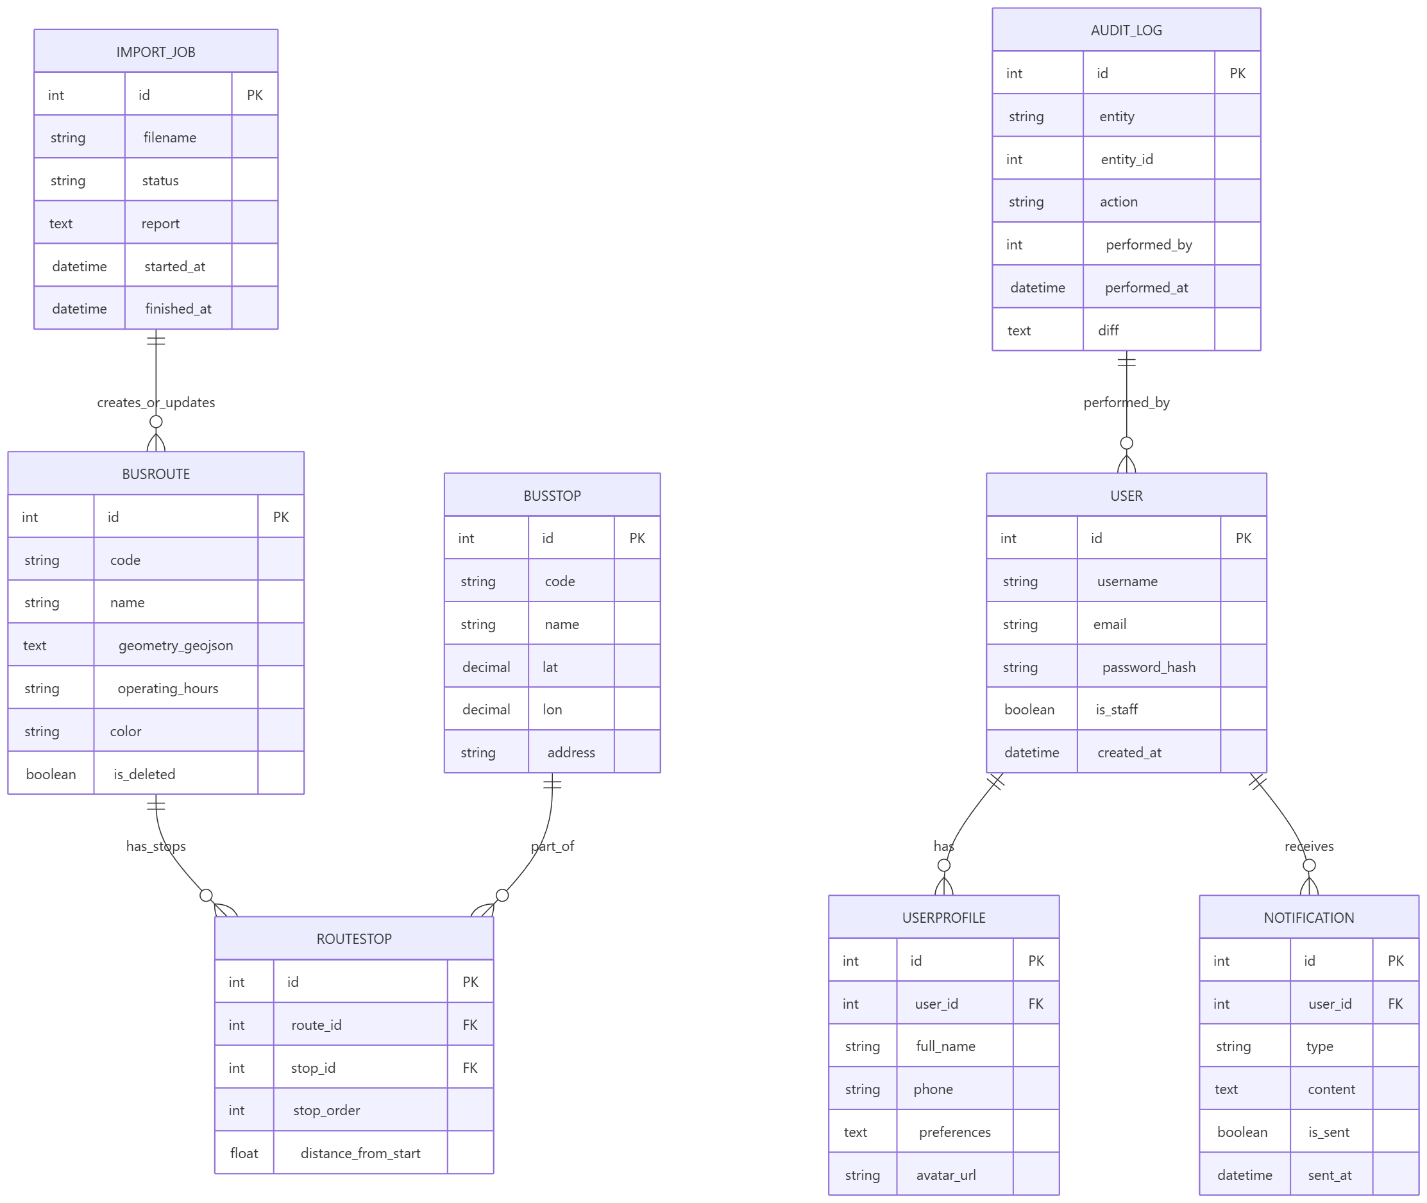
\includegraphics[width=\textwidth]{images/image5.png}
    \caption{Giao diện Trang chủ Bản đồ tương tác}
\end{figure}

Tại đây, người dùng có thể kéo thả, phóng to, thu nhỏ và nhấn chọn trực tiếp vào các biểu tượng điểm dừng (Markers) để xem tên trạm, địa chỉ. Hệ thống cũng cung cấp thanh tìm kiếm nhanh để xác định ngay vị trí một địa điểm cụ thể trên bản đồ.

\subsection{Danh mục truy xuất Tuyến xe buýt và Trạm dừng}

Tính năng truy xuất tuyến xe cho phép liệt kê toàn bộ mạng lưới xe buýt dưới dạng danh sách các thẻ thông tin (Cards). Mỗi thẻ hiển thị rõ ràng số tuyến, tên điểm đầu cuối và nhãn trạng thái hoạt động.

\begin{figure}[H]
    \centering
    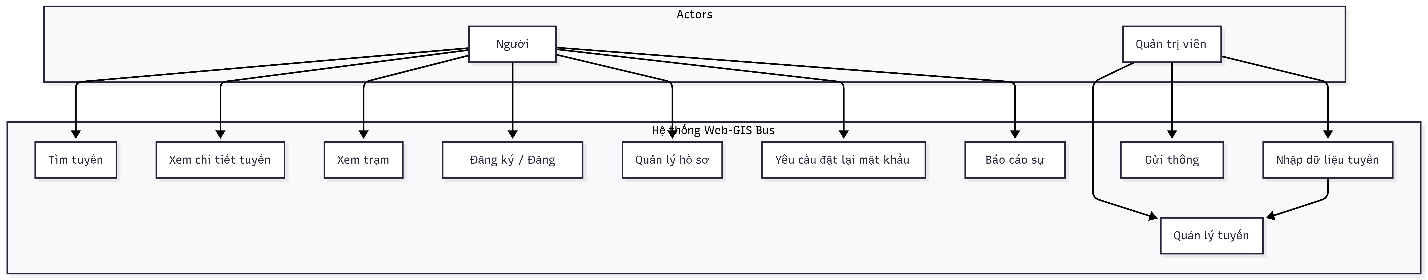
\includegraphics[width=\textwidth]{images/image6.png}
    \caption{Giao diện Danh sách các tuyến xe buýt}
\end{figure}

Giao diện còn hỗ trợ phân trang (Pagination) để tối ưu thời gian tải trang đối với các danh sách dài. Đối với danh sách Trạm dừng, người dùng có thể áp dụng các bộ lọc tiện ích như "Có mái che", "Có ghế ngồi" để sàng lọc kết quả hiển thị mong muốn.

\subsection{Chi tiết thông tin cấu trúc một Tuyến xe cụ thể}

Khi người dùng nhấn chọn một tuyến xe, hệ thống sẽ chuyển hướng sang Trang Chi tiết Tuyến. Tại đây, toàn bộ thông tin giá vé, thời gian hoạt động và tần suất được trình bày trực quan.

\begin{figure}[H]
    \centering
    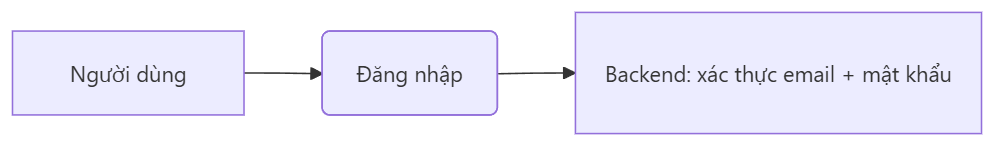
\includegraphics[width=\textwidth]{images/image7.png}
    \caption{Giao diện Chi tiết Tuyến và Dòng thời gian Trạm dừng}
\end{figure}

Một thành phần nổi bật trong giao diện này là dải Dòng thời gian (Timeline) hiển thị thứ tự các trạm mà tuyến xe đi qua. Đồng thời, hệ thống cung cấp tính năng Xem đánh giá (Reviews), nơi hành khách có thể để lại bình chọn 1-5 sao và nhận xét cá nhân về chất lượng phục vụ của tuyến.

\section{Nhóm công cụ Phân tích Không gian (GIS Tools)}

\subsection{Tra cứu và tìm hướng đi định tuyến (Routing)}

Tính năng cốt lõi giúp phân biệt BusGIS với các website tra cứu thông thường là công cụ định tuyến tự động. Bằng cách chọn điểm xuất phát và điểm đến trên bản đồ, công cụ tính toán sẽ sử dụng thuật toán phân tích mạng lưới tuyến để đề xuất lộ trình phù hợp, bao gồm các điểm trung chuyển nếu cần chuyển tuyến.

\begin{figure}[H]
    \centering
    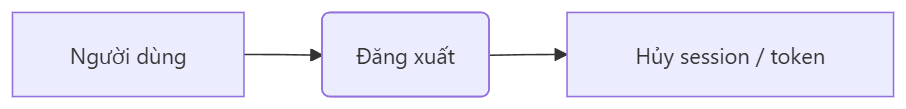
\includegraphics[width=\textwidth]{images/image8.png}
    \caption{Công cụ Tìm kiếm Định tuyến xe buýt}
\end{figure}

Kết quả được vẽ trực tiếp bằng các dải màu nổi bật trên bản đồ không gian, kèm theo bảng hướng dẫn di chuyển chi tiết từng chặng phía bên lề trái màn hình.

\subsection{Đánh giá không gian mạng lưới dịch vụ (Buffer Zone)}

Chức năng tạo vùng đệm (Buffer Zone) cho phép phân tích phạm vi bao phủ của mạng lưới giao thông. Người dùng chọn một trạm dừng và thiết lập bán kính (ví dụ 500m hoặc 1km), hệ thống sẽ vẽ một vòng tròn bao quanh trạm trên bản đồ.

\begin{figure}[H]
    \centering
    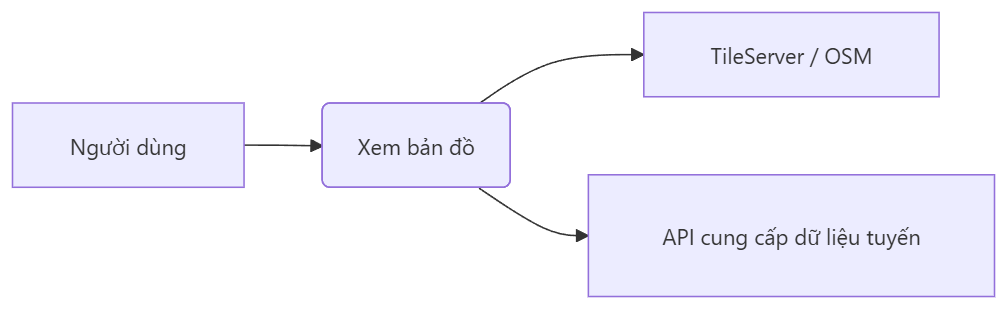
\includegraphics[width=\textwidth]{images/image9.png}
    \caption{Phân tích vùng đệm phục vụ của Trạm xe buýt}
\end{figure}

Tính năng này hỗ trợ đắc lực trong việc đánh giá mức độ tiếp cận giao thông công cộng tại khu vực cư dân cụ thể, hỗ trợ công tác quy hoạch điểm đặt trạm mới cho cơ quan quản lý.

\section{Phân hệ Xác thực hệ thống và Chiến lược Bảo mật}

Hệ thống BusGIS quản lý quyền truy cập thông qua mô hình phân quyền chặt chẽ. Trang Đăng nhập (Login) và Đăng ký (Register) được thiết kế hiện đại, thông báo lỗi rõ ràng. 

\begin{figure}[H]
    \centering
    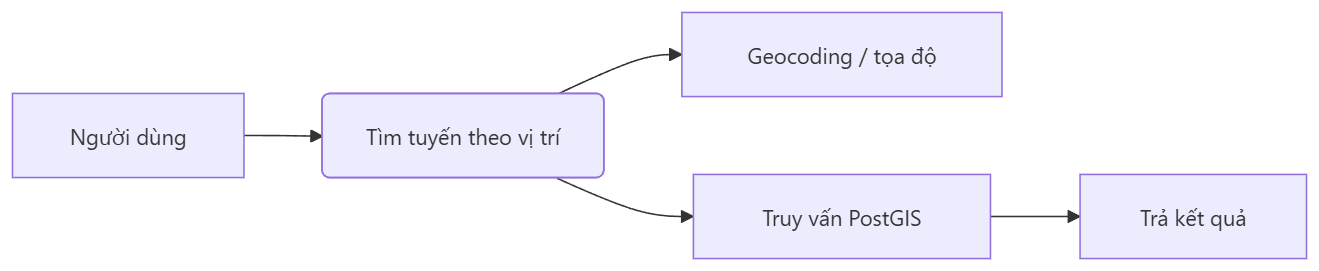
\includegraphics[width=\textwidth]{images/image10.png}
    \caption{Giao diện Xác thực người dùng}
\end{figure}

Sau khi xác thực, người dùng sở hữu không gian Quản lý Hồ sơ cá nhân (Profile) để cập nhật thông tin. Đặc biệt đối với các tài khoản thuộc cấp Quản trị (Admin/Staff), hệ thống tự động mở khóa liên kết đến Bảng điều khiển Quản lý nội bộ (Management Dashboard). Tại đây, quản trị viên có thể giám sát số lượng tài khoản đăng ký mới, thực hiện thêm/sửa/xóa tuyến xe và xuất báo cáo dữ liệu định dạng Excel.
